\chapter{Конструкторская часть}
В этом разделе будут представлены схемы алгоритмов построения деревьев синтаксических зависимостей в тексте с распараллеливанием и без него.

\section{Требования к программному обеспечению}

К программе предъявлен ряд требований:
\begin{enumerate}[label=\arabic*)]
	\item иметь интерфейс для выбора действий;
	\item работать с «нативными» потоками;
	\item замерять процессорное время работы реализаций алгоритмов.
\end{enumerate}

\section{Разработка алгоритмов}

На рисунках \ref{fig:noparal}, \ref{fig:paral} и \ref{fig:one_paral} представлены схемы алгоритмов построения дерева синтаксических зависимостей в тексте без многопоточности и с ней соответственно, а также схема алгоритма одного рабочего потока для варианта с многопоточностью.

\begin{figure}[h!]
	\centering
	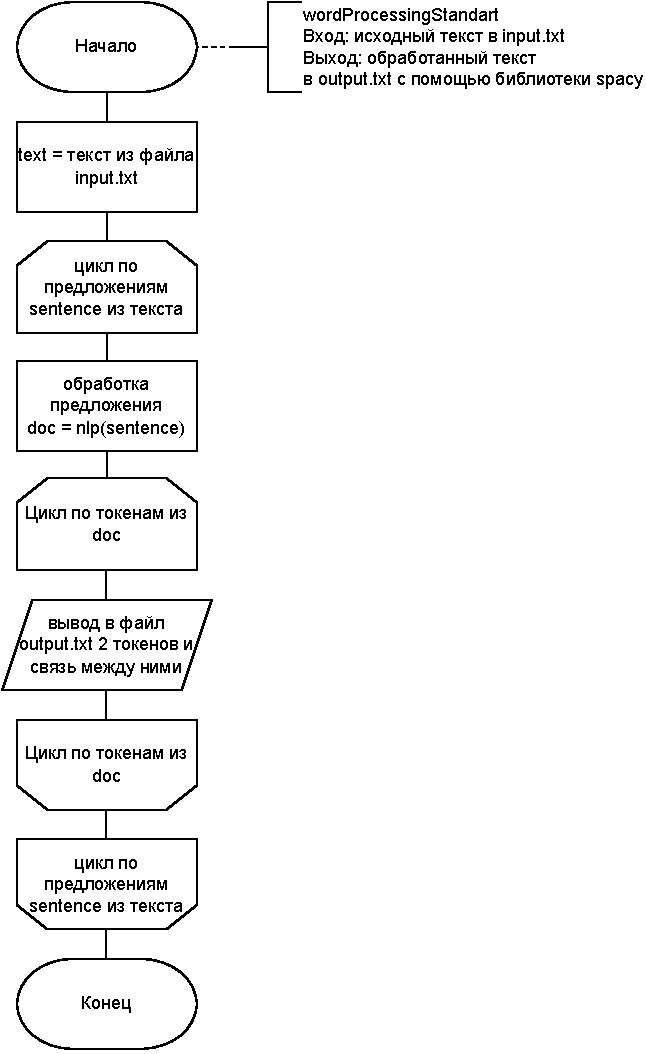
\includegraphics[width=0.5\linewidth]{img/no_paral}
	\caption{Схема алгоритма построения деревьев синтаксических зависимостей в тексте (без многопоточности)}
	\label{fig:noparal}
\end{figure}

\begin{figure}[h!]
\centering
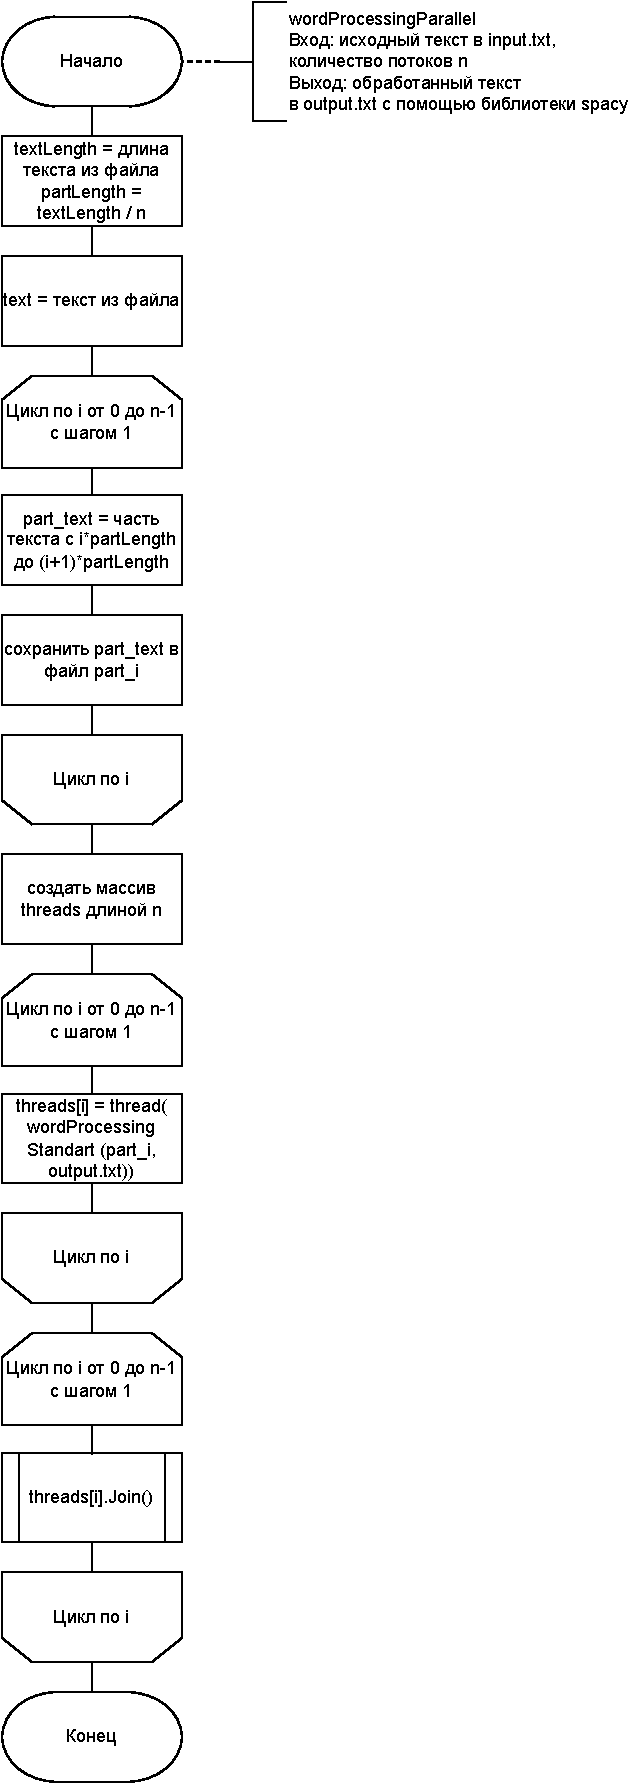
\includegraphics[width=0.5\linewidth]{img/paral}
\caption{Схема алгоритма построения деревьев синтаксических зависимостей в тексте (с многопоточностью)}
\label{fig:paral}
\end{figure}

\begin{figure}[h!]
	\centering
	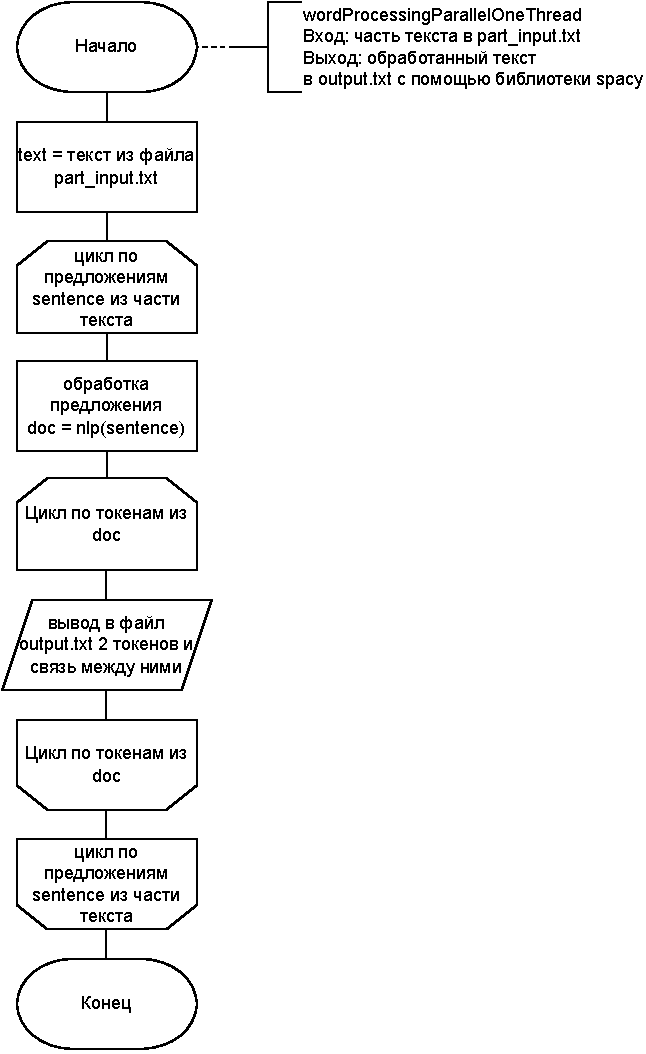
\includegraphics[width=0.5\linewidth]{img/one_paral}
	\caption{Схема алгоритма одного рабочего потока для варианта с многопоточностью}
	\label{fig:one_paral}
\end{figure}


\clearpage

\section*{Вывод}

В данном разделе были представлены схемы алгоритмов построения деревьев синтаксических зависимостей в тексте с распараллеливанием и без него.